\subsection{Fragekatalog}
Der Fragekatalog wurde für das Interview mit einer anderen Unternehmung aufgebaut.
Die einzelnen Themenblöcke und die Zusammenstellung der Fragen wurden
gezielt auf die Struktur der bestehenden Analyse der allink zusammengestellt um einen
möglichst guten Vergleich darstellen zu können.

\newcounter{qcounter}
\begin{center}
    \begin{longtable}{lp{14cm}}
        \toprule \textbf{Nr.} & \textbf{Frage} \\
        \midrule & \textbf{Allgemeine Fragen} \\
        \midrule \addtocounter{qcounter}{1}\arabic{qcounter} & Wer ist mein Interviewpartner? \\
        \midrule \addtocounter{qcounter}{1}\arabic{qcounter} & Was ist die Funktion meines Interviewpartners? \\
        \midrule \addtocounter{qcounter}{1}\arabic{qcounter} & Was sind die Aufgaben meines Interviewpartners? \\
        \midrule & \textbf{Unternehmen} \\
        \midrule \addtocounter{qcounter}{1}\arabic{qcounter} & Wann wurde das Unternehmen gegründet? \\
        \midrule \addtocounter{qcounter}{1}\arabic{qcounter} & Wie viele Partner mit Mitspracherecht existieren? \\
        \midrule \addtocounter{qcounter}{1}\arabic{qcounter} & Wie ist das Organigramm des Unternehmens aufgebaut? \\
        \midrule \addtocounter{qcounter}{1}\arabic{qcounter} & Wie viele Vollzeitangstellte werden beschäftigt? \\
        \midrule \addtocounter{qcounter}{1}\arabic{qcounter} & Sind Praktikanten angestellt? \\
        \midrule \addtocounter{qcounter}{1}\arabic{qcounter} & Bietet das Unternehmen Lehrstellen an? \\
        \midrule & \textbf{Kunden} \\
        \midrule \addtocounter{qcounter}{1}\arabic{qcounter} & Wie viele Kunden sind Kleinstunternehmen? \\
        \midrule \addtocounter{qcounter}{1}\arabic{qcounter} & Wie viele Kunden sind kleine Unternehmen? \\
        \midrule \addtocounter{qcounter}{1}\arabic{qcounter} & Wie viele Kunden sind mittlere Unternehmen? \\
        \midrule \addtocounter{qcounter}{1}\arabic{qcounter} & Wie viele Kunden sind grosse Unternehmen? \\
        \midrule & \textbf{Projektablauf} \\
        \midrule \addtocounter{qcounter}{1}\arabic{qcounter} & Wie viele Projekte werden akquiriert? \\
        \midrule \addtocounter{qcounter}{1}\arabic{qcounter} & Wie viele Projekte entstehen durch direkte Anfragen? \\
        \midrule \addtocounter{qcounter}{1}\arabic{qcounter} & Wie werden die Aufwände eines potenziellen Projektes geschätzt? \\
        \midrule \addtocounter{qcounter}{1}\arabic{qcounter} & Wie wird auf Änderungen während des Projektes reagiert? \\
        \midrule \addtocounter{qcounter}{1}\arabic{qcounter} & Kommt es vor, dass Projekte während der Durchführung abgebrochen werden? \\
        \midrule \addtocounter{qcounter}{1}\arabic{qcounter} & Von wem werden die Arbeitspakete zusammengestellt? \\
        \midrule \addtocounter{qcounter}{1}\arabic{qcounter} & Wie werden die Arbeitspakete verteilt? \\
        \midrule \addtocounter{qcounter}{1}\arabic{qcounter} & Wie werden die Aufwände rapportiert? \\
        \midrule \addtocounter{qcounter}{1}\arabic{qcounter} & Wer kommuniziert direkt mit einem Kunden? \\
        \midrule \addtocounter{qcounter}{1}\arabic{qcounter} & Wie wird das Feedback eines Kunden verarbeitet? \\
        \midrule \addtocounter{qcounter}{1}\arabic{qcounter} & Wie wird mit zusätzlich zu verrechneten Anforderungen verfahren? \\
        \midrule \addtocounter{qcounter}{1}\arabic{qcounter} & Wie werden die Projektdaten archiviert? \\
        \midrule & \textbf{Verwendete Software} \\
        \midrule \addtocounter{qcounter}{1}\arabic{qcounter} & Auf welches Betriebssystem setzt das Unternehmen? \\
        \midrule \addtocounter{qcounter}{1}\arabic{qcounter} & Welche Office Suite setzt das Unternehmen ein? \\
        \midrule \addtocounter{qcounter}{1}\arabic{qcounter} & Was für Projektmanagement-Software wird verwendet? \\
        \midrule & \textbf{Stärken und Schwächen} \\
        \midrule \addtocounter{qcounter}{1}\arabic{qcounter} & Wo liegen die Stärken des Unternehmens? \\
        \midrule \addtocounter{qcounter}{1}\arabic{qcounter} & Wo sieht das Unternehmen ihre Chancen? \\
        \midrule \addtocounter{qcounter}{1}\arabic{qcounter} & Wo liegen die Schwächen des Unternehmens? \\
        \midrule \addtocounter{qcounter}{1}\arabic{qcounter} & Mit was für Risiken sieht sich das Unternehmen konfrontiert? \\
        \bottomrule
        \caption{Fragekatalog zur Marktanalyse}
        \label{tab:fragekatalog}
    \end{longtable}
\end{center}

Der erstellte Fragenkatalog dient als Leitfaden im Interview. Die Antworten
werden entgegengenommen, diskutiert und anschliessend in beschreibender Form
dokumentiert und mit allink verglichen. 

\subsection{Unternehmen}
Das Unternehmen Panter IIc mit Sitz in Zürich hat sich freundlicherweise dazu
bereiterklärt mit dem Studierenden ein Interview durchzuführen.

\subsection{Kunden}

\begin{figure}[htbp]
\begin{center}
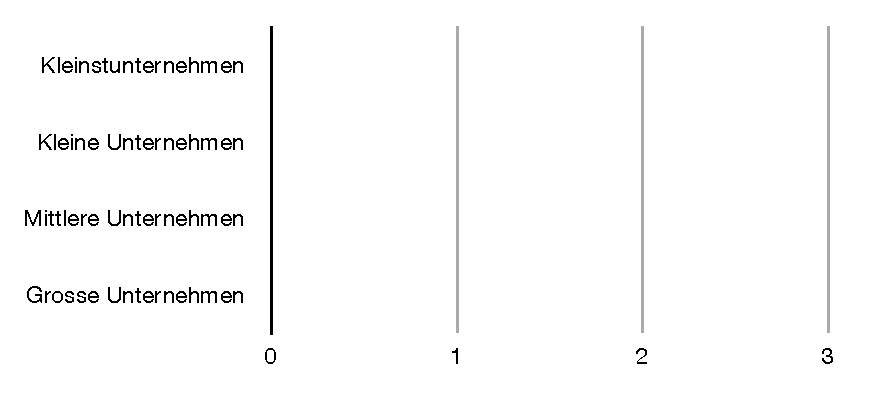
\includegraphics[width=0.75\textwidth,angle=0]{./bilder/analyse/marktanalyse/kundenkategorisierung.pdf}
\caption{Anzahl Kunden von Panter in Unternehmensgrössen kategorisiert}
\label{pic:kundenkategorisierung_panter}
\end{center}
\end{figure}

\subsection{Projektablauf}

\subsubsection{Projektannahme und Offertenstellung}

\subsubsection{Projektdurchführung}

\subsubsection{Projektabschluss}

\subsection{Verwendete Software}

\begin{center}
    \begin{longtable}{lllp{6cm}}
        \toprule \textbf{Bezeichnung} & \textbf{Hersteller} & \textbf{Kategorie} & \textbf{Verwendungszweck} \\
        \midrule ... & ... & ... & 
            \begin{minipage}[t]{6cm}
                \begin{compactitem}
                    \item ...
                \end{compactitem}
            \end{minipage}
            \\\\
        \bottomrule
        \caption{Verwendete Software bei Panter}
        \label{tab:verwendete_software_panter}
    \end{longtable}
\end{center}

\subsubsection{...}

\subsection{Stärken und Schwächen}

\begin{figure}[htbp]
\begin{center}
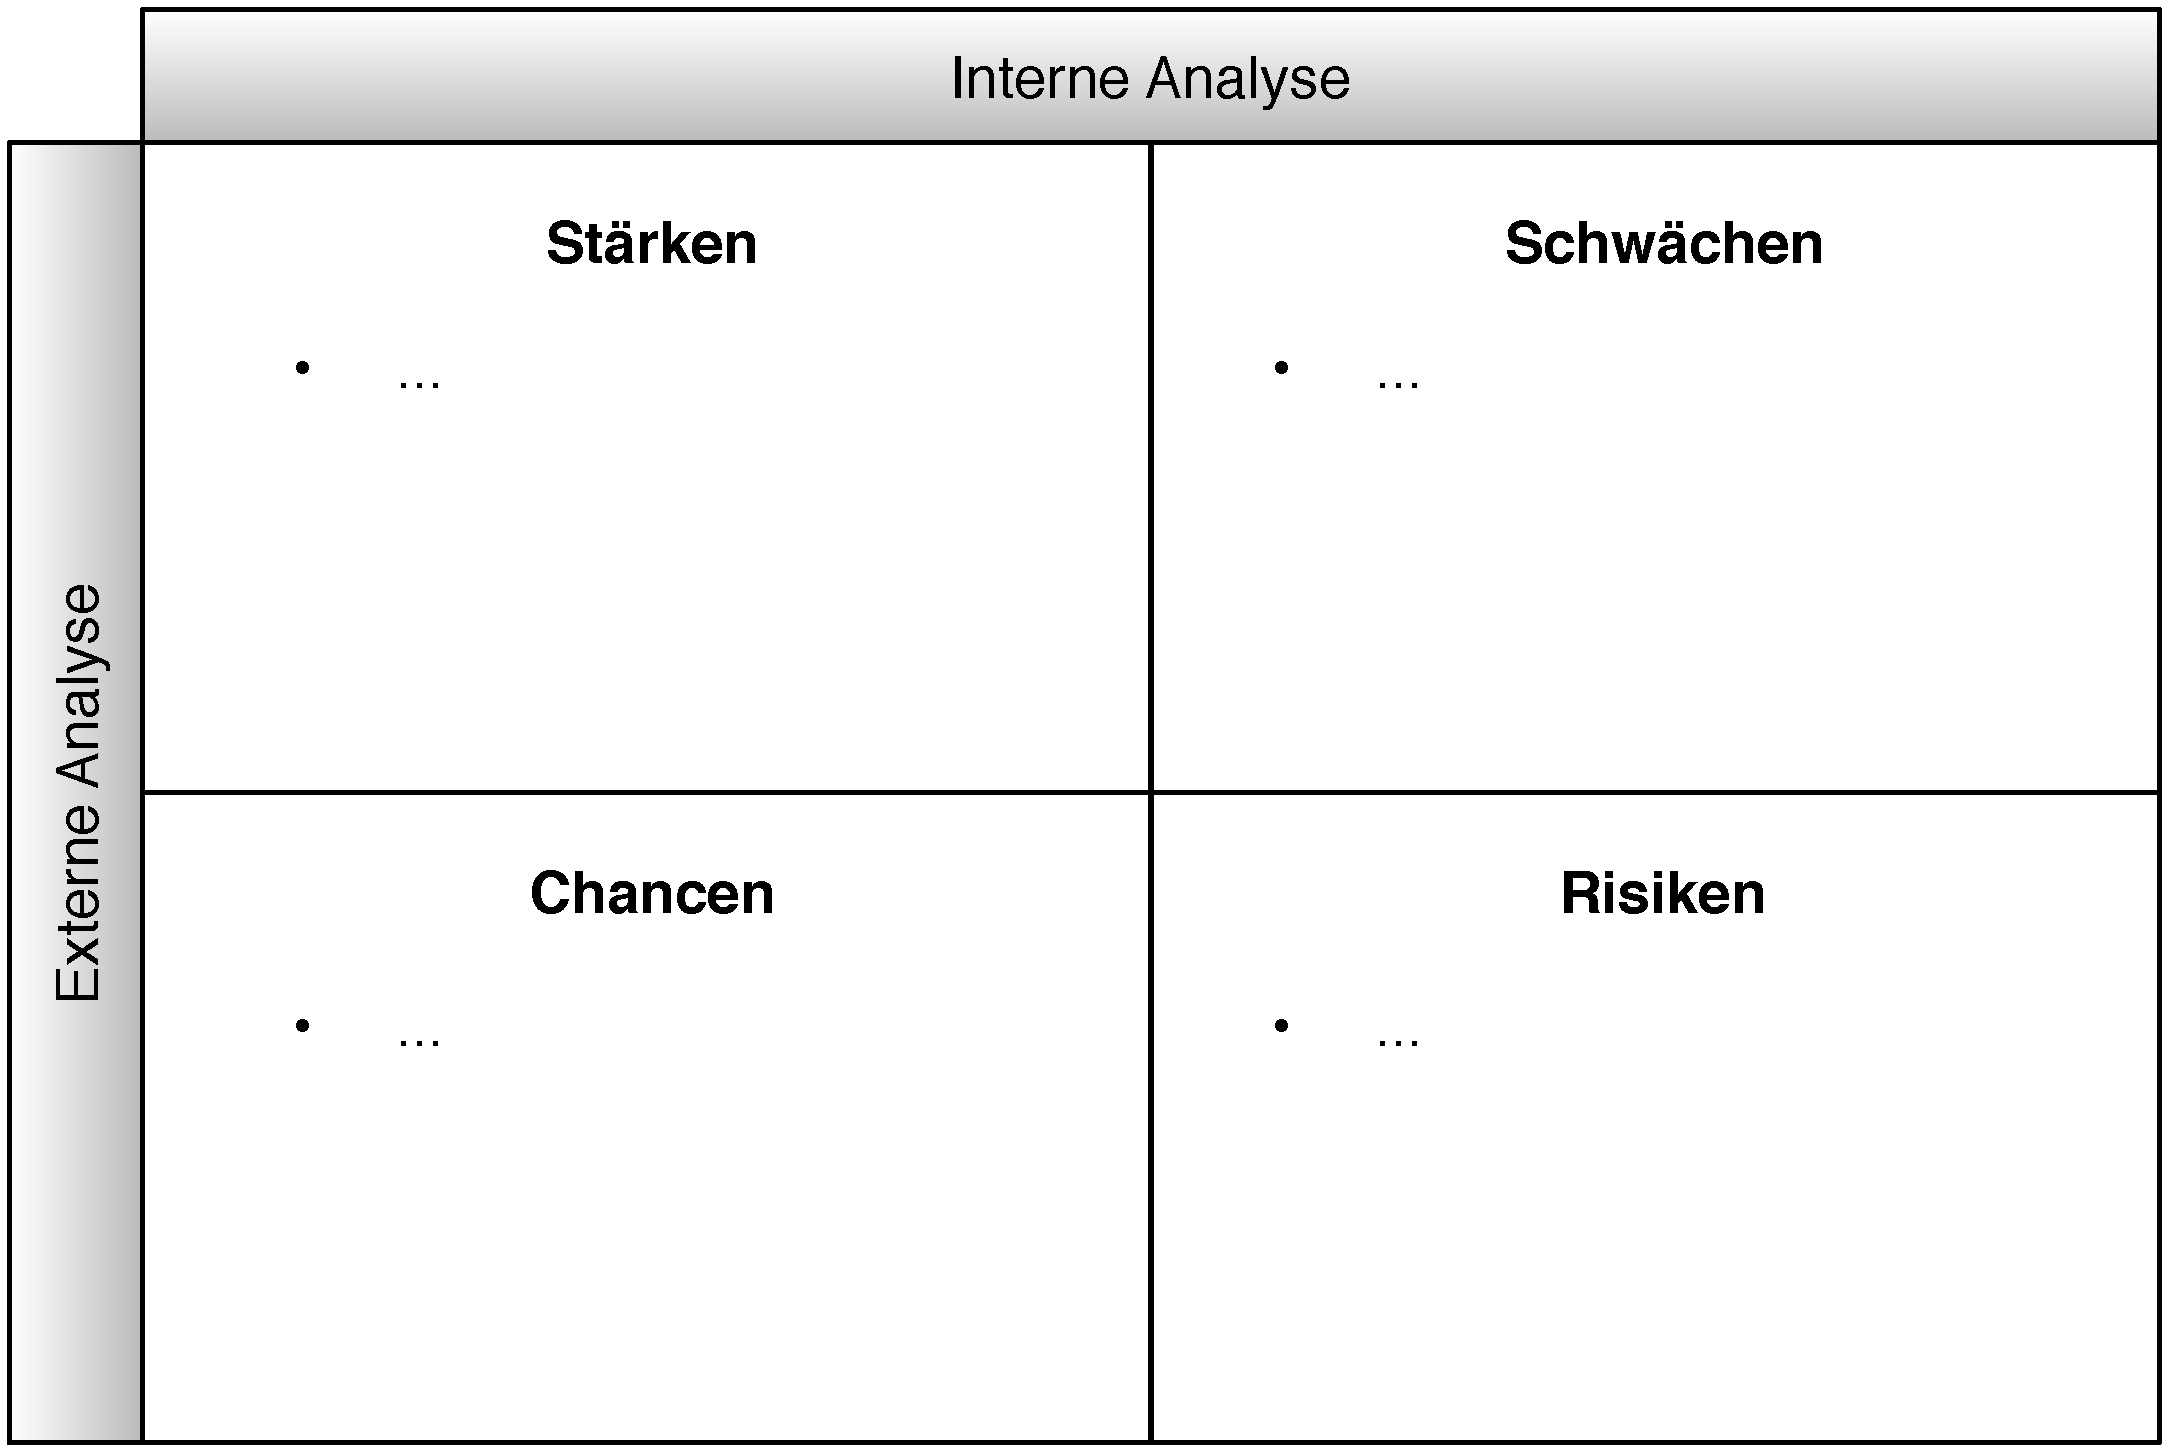
\includegraphics[width=0.8\textwidth,angle=0]{./bilder/analyse/marktanalyse/swot_analyse.pdf}
\caption{SWOT-Analyse von Panter}
\label{pic:swot_analyse_panter}
\end{center}
\end{figure}